\chapter{Planification et demande}

\begin{center}
    \makebox[\textwidth]{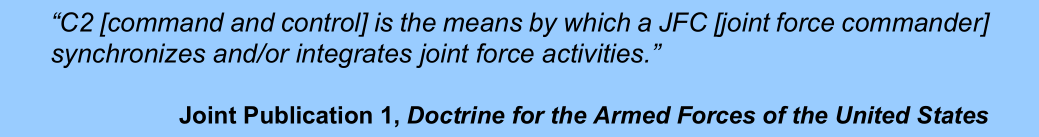
\includegraphics[width=\paperwidth]{quote3.png}}
\end{center}

\e
    \item Il existe deux types de \gls{cas} distincts:
    \ee
        \item Le \gls{cas} planifié
        \item Le \gls{cas} immédiat
    \ed
\ed

\section{Le CAS planifié}

\e
    \item Le ``\gls{cas} request'' est effectué par l'unité qui demande un soutien aérien. On distingue deux principaux types de demandes:
    \ee
        \item Le \gls{cas} planifié à l'avance (``pre-planned \gls{cas}'', ou simplement ``\gls{cas}'')
        \item Le \gls{cas} ``à la demande'' (``on-call cas''), qui regroupe deux possiblités:
        \eee
            \item Le \gls{xcas}, où l'appareil en attente de tasking se trouve déjà dans les airs
            \item Le \gls{gcas}, où l'appareil en attente de tasking se trouve encore au sol
        \ed
    \ed
    \item Un ``\gls{cas} request'' réel se compose d'un grand nombre d'informations, utiles à la planification de la mission et à la répartition des effectifs disponibles.
    \item
    Souvent, pour DCS, l'équivalent du ``\gls{cas} request'' sera contenu dans le briefing de la mission (zone d'opération, menace, composition et force de unités ennemies, timing, emport, unités amies, \gls{jtac}, plan de fréquences, etc…).
    \item Toute référence ultérieure au ``\gls{cas} request'' fera donc implicitement référence au briefing de mission.
    \item Les considération à prendre en compte lors de l'établissement d'une \gls{cas} request sont propres au rôle de \gls{gc}/\gls{jfc} et ne seront pas traitées dans ce document.
    \item Le \gls{cas} planifié est un \gls{cas} effectué après une requête spécifique, concernant une zone connue, pour atteindre un objectif déterminé.
    \item Dans le cas d'un \gls{cas} planifié, un grand nombre de paramètres sont connus avant le décollage, ce qui permet une meilleure préparation.
\ed

\subsection{Étape 1: réception de l'ordre de mission}

\e
    \item
    En tant que participants au processus de planification, les officiers en charge (chef de patrouille, commandant d'escadron, …) devraient être à même de comprendre et analyser l'information à partir de ces différentes sources:
    \ee
        \item \gls{aob}
        \item \gls{ato}
        \item \gls{aco}
        \item \gls{spins}
        \item \gls{opord}
        \item \gls{sop}
    \ed
\ed
\note{Les \glspl{sop} sont propres à l'escadron, et sont normalement connues par les tous les officiers supérieurs.
    
    Exceptés les \glspl{sop}, tous les éléments sont normalement fournis sous une forme ou l'autre dans le briefing de mission.
    
    S'il devait manquer un élément, il appartient à l'officier en charge de la patrouille d'évaluer son importance et de poser les questions nécessaires à l'organisateur de la mission.
}

\subsection{Étape 2: analyse de la mission} 

\e
    \item Avant de pouvoir préparer la mission, les officiers en charges devront:
    \ee
        \item Mettre à jour les différentes sources d'informations (\gls{ato}, \gls{spins}, \gls{aco}, …)
        \item Estimer les capacités des forces à leur disposition (équipement, personnel, restrictions, …)
        \item Déterminer les tâches essentielles de la mission
        \item Évaluer les conditions relatives à:
        \eee
            \item L'ennemi
            \item La météo
            \item Le terrain
        \ed
        \item Avertir les unités (personnes) subordonnées
    \ed
    \item Considérations clefs à prendre en compte lors de l'analyse de la mission:
    \ee
        \item \gls{conops}: Quelles sont les intentions du \gls{jfc}? Attaque ou de défense? Surprise ou délibéré? Règles d'engagement?
        \item Comment s'intègre le \gls{cas} au reste du dispositif?
        \item Quelles pourraient être les intentions de l'ennemi? Comment ces intentions sont-elles affectées par le terrain, la météo, l'heure ?
        \item Quels sont les moyens de surveillance ou de reconnaissance à notre disposition?
        \item \gls{complan} Comment vont s'organiser les communications? Est-ce que toutes les unités participantes au \gls{cas} sont intégrées au \gls{complan}  de manière fiable et redondante?
    \ed
    \item Dans le cas d'une demande de \gls{cas} pré-planifié, un grand nombre d'informations supplémentaires pourront être obtenues via la demande elle-même. Par exemple:
    \ee
        \item Zone de \gls{cas}
        \item Menaces
        \item Type de cibles
        \item Localisation de la cible
        \item Localisation des forces amies
        \item Type de terrain
        \item Restrictions horaires
        \item \gls{jtac}
    \ed
\ed

\subsection{Étape 3: préparation de la mission}

\begin{center}
    \makebox[\textwidth]{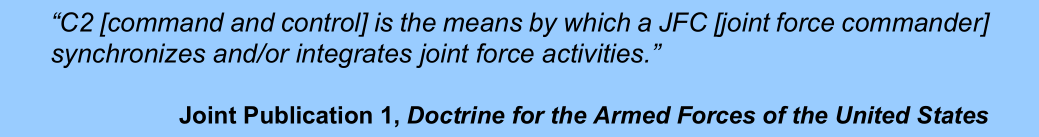
\includegraphics[width=\paperwidth]{quote2.png}}
\end{center}

\e
    \item Le ``Mission planning'', ou ``préparation de la mission'', est une étape cruciale au bon déroulement de cette dernière.
    \item Cette préparation sera effectuée par le chef de patrouille, qui sera chargé de rassembler et analyser toutes les informations à sa disposition pour préparer au mieux la mission de la patrouille dont il a la charge.
    \item Lorsque c'est possible, la préparation de la mission se fait en collaboration avec les différents éléments impliqués, certainement avec le \gls{jtac} en charge de la zone attribuée à la patrouille, le \gls{tacon}, et les autres chefs de patrouilles opérant dans le même théâtre opérationnel.
    \item Le chef de patrouille veillera tout particulièrement à toujours utiliser les informations les plus récentes, et fera attention à se tenir au courant de l'évolution de la situation.
    \item Il devra également s'assurer que tous les éléments sous son contrôle ont reçu et compris ses intentions pour la mission.
    \item Checklist de préparation de mission: \fullref{ann1}
\ed

\section{Le CAS immédiat}

\e
    \item Le \gls{cas} immédiat intervient lorsque la situation sur le champ de bataille évolue de manière inattendue.
    \item L'\gls{ato} peut allouer un certain effectif pour se préparer à répondre à ces situations.
    \item Le chef de patrouille trouvera alors dans cet \gls{ato} les informations nécessaires pour préparer son vol (emport, point d'attente, etc…).
    \item
    Pendant le vol (ou au parking pour le \gls{gcas}), si l'intervention de la patrouille s'avère nécessaire, celle-ci recevra un point de contact initial, ainsi que le call-sign et la fréquence de l'agence qui s'occupera de son contrôle terminal.
\ed





